\section{Før Barvagten}
\label{sec:pre-barvagten}

Vi mødes 14.30 ved gitteret. Baren åbner kl 15.00

Før barvagten, skal baren sættes op med alt hvad det indebærer. Her er
det sorteret efter, hvorfra ting skal hentes/ting skal ordnes.

Under barvagten har du som bartender adgang til en \textit{bar-nøgle}\index{bar-nøgle}. 
Denne nøgle ligger i baren og kan låse op til \textit{Bag Gitteret}\index{Bag Gitteret}, 
\textit{Rummet under Trappen}\index{Rummet under Trappen}, \textit{Træburet}\index{Træburet} i Hopper -1, 
lageret i \textit{Parkeringskælderen}\index{Parkeringskælderen} og 
\textit{Rengøringsrummet}\index{Rengøringsrummet} overfor handicaptoiletterne i Nygaard -1.

Baren lukker normalt kl. 22:00, men kan evt. lukkes tidligere, hvis der ikke er mange kunder.
Ved fester eller lign. kan vi dog lukke senere, dette vil blive varslet i forvejen og der vil 
være flere hold bartendere tilknyttet en sådan vagt.

\subsection{Bag Gitteret}
\label{sec:pre:bag-ved-gitteret}

\begin{itemize}
	\item Baren skal køres hen til barområdet med tilhørende \textit{drypspand}\index{drypspand}.
	\item \textit{Køleskabene}\index{Køleskabene} skal være fyldte, og køres hen på hver sin side af køleskabene i 
	Barområdet\index{Barområdet}.
	\item Tomme plastkopper i opvaskebakke hentes.
	\item Papkassen til pant hentes.
	\item Hvis det er den første fredag i måneden, så tag også lykkehjulet frem.
\end{itemize}

\subsection{Parkeringskælderen}
\label{sec:pre:hopper}

\begin{itemize}
	\item Der skal hentes fustager i Parkeringskælderen. Normalt 1
	Extra Pilsner, 1 cider og 1 specialøl\footnote[1]{\label{note1}Det handler bare om ikke at løbe
	tør.}.
	\item Derudover skal der hentes flaskeøl. Normal 2 kasser Top, 2 kasser Classic, 
	1 kasse Grøn og 1 kasse Sport Cola \footnotemark[1].
\end{itemize}

\subsection{Under Trappen}
\label{sec:pre:under-trappen}

\begin{itemize}
	\item Chips skal hentes.
	\item \textit{Ståmåtte}\index{Ståmåtte} skal hentes.
	\item \textit{Brætspil}\index{Brætspil} skal hentes.
	\item Kasserne med spiritus, shotglas og shotsbakker skal hentes.
\end{itemize}

\subsection{Barområdet}
\label{sec:pre:baromradet}

\begin{figure}[H]
	\centering
	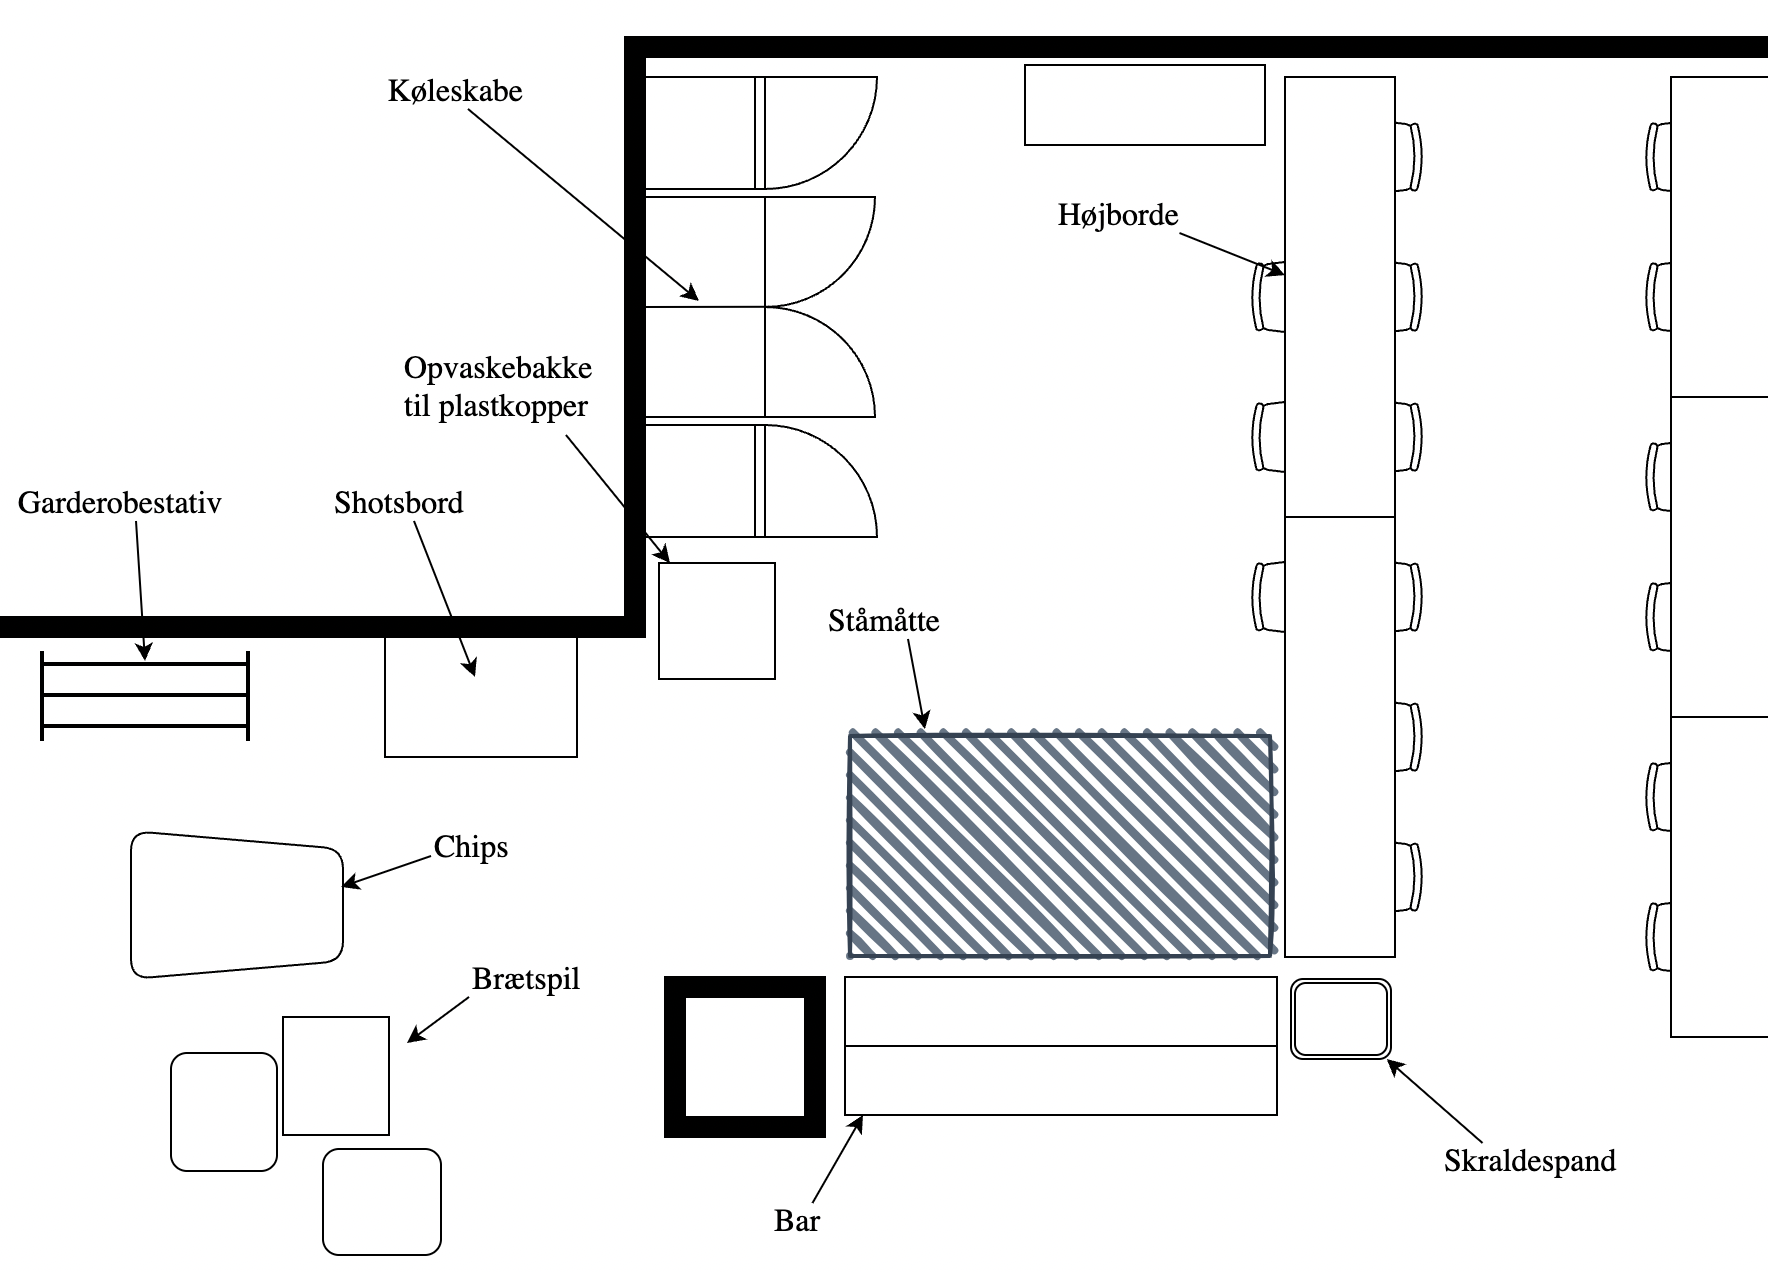
\includegraphics[width=\linewidth]{billeder/baromraadet_w_labels.png}
	\caption{Barområdet}
	\label{fig:baromraadet}
\end{figure}

\begin{itemize}
	\item Der sluttes strøm til køleskabene. Tænd gerne lyset i de nye køleskabe, men ikke i de gamle, 
	da lysene her har det med at blive varme.
	\item Efter baren er kørt på plads, sættes de to barborde op, og der sættes barstole op omkring dem.
	\item Der sættes sorte affaldssække op, hvis der ikke allerede er. 
		Det er en god ide at have en skraldespand ved baren.
	\item Baren skal sluttes til strøm.
	\item Fustager skal sluttes til, og der skal tændes for gassen:
	\begin{itemize}
		\item Pilsner sluttes til de yderste haner (1 fustage dækker begge
		haner).
		\item Cider sluttes til midt-venstre hane.
		\item Specialøl sluttes til midt-højre hane.
	\end{itemize}
	\item En affaldssæk placeres under opvaskebakken til brugte plastkopper.
	\item iPaden skal tilsluttes \textit{eduroam}\index{eduroam}.
\end{itemize}

\subsection{Rengøringsrummet}
\label{sec:pre:rengøring}
\begin{itemize}
	\item Fra Rengøringsrummet kan man med fordel hente en spand med sæbevand og en klud.
	\item Derudover findes der en nøgle oven i papirdispenseren. Denne kan man bruge til 
	at åbne ind til rullen, og man kan med fordel hente en rulle ``\textit{Spæns}\index{Spæns}'' 
	fra et af de åbne toiletter. Husk at fjerne det blå stykke plastik i enden.
\end{itemize}